%!TEX root = ../vernier.tex
\section{Linking the Views} \label{sec:linking}
So far we have three views. A projection view on the left, a hierarchical view on the right, that by default displays the Squarified Treemap, and if solicited through the UI, an evolution view on the bottom.

Selecting or brushing elements or groups of elements on one of the views, highlights them on the others. This is a simple mechanism that attempts to support the visualization of correlation between $\mathbb{R}^{n}$ similarity, project structure and metric evolution. Its downside is that it relies on having to move the user's attention from one view to the next. In this section, we experiment with ways of hinting information about hierarchy on top of the projection (which as far as we are concerned, no one has attempted to on the literature) and vice versa.

For the projection, we've developed a technique based on force-directed graph layout that links each class to its hierarchical parent. Points in the projection (i.e. classes) are constrained to their original $\mathbb{R}^{2}$ positions (leaf nodes) and package representative nodes are free to move according to the forces acting upon them (non leafs).

In this graph, each class point connects to its package representative. In turn, every package representative node connects to the tree root node.

Each node is capable of generating attraction and repulsion forces. Two linked nodes attract each other with a force linearly proportional to their distance. Additionally, each node repels all other nodes with a force that degrades quadratically with their pair-wise distance and is scaled by the node's radius in order to try to avoid overlap.

If a node is able to move (i.e. package representative or root), the sum of the forces acting upon it as well as its current velocity dictate its position on the next iteration, creating a system that simulates particle momentum. This system iterates until it reaches equilibrium, which is only broken when we move to the next revision and node positions change. In which case, the system smoothly transitions to a new stable configuration.

Figure \ref{fig:hier_graph_synth} is an example of a stable configuration for a simple hierarchy. Figure \ref{fig:hier_sim_graph} shows the same scenario for a more complex dataset (117 classes). With this number of classes it is already impossible to get any hierarchical insight. But if we are only interested in understanding the $\mathbb{R}^{n}$ neighborhood of a couple of packages, figure \ref{fig:hier_two_sim_graph} shows that it is possible to do so through filtering.

\begin{figure}[H]
	\centering
	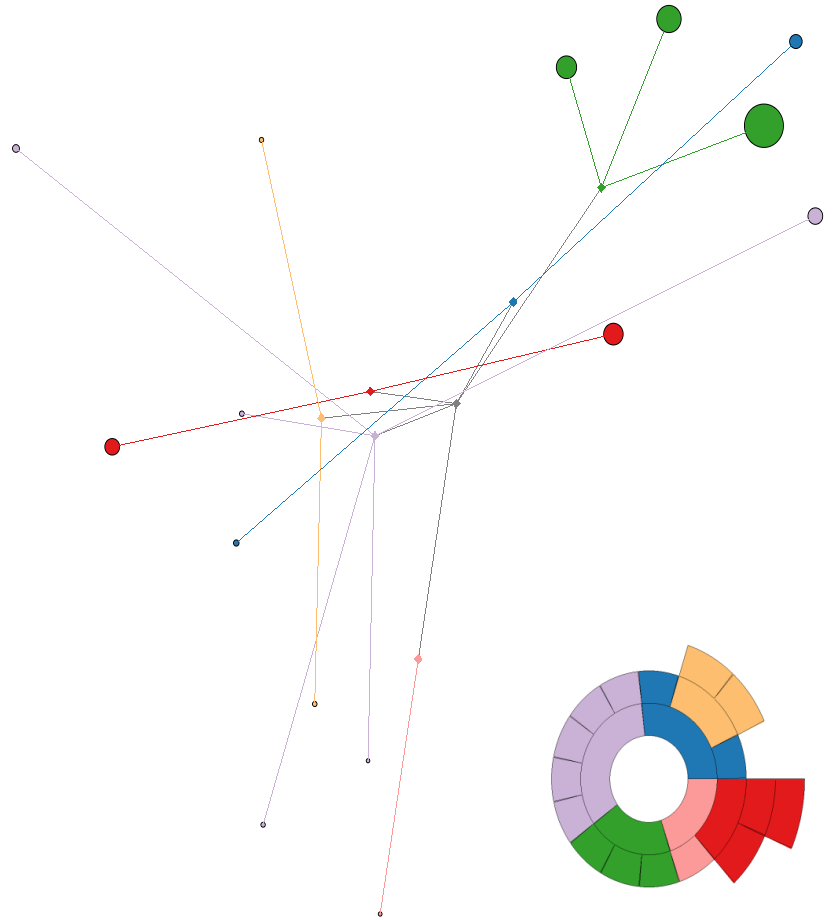
\includegraphics[width=0.7\textwidth]{figures/hier_graph_synth.png}
	\caption{Linking nodes hierarchically on a synthetic projection}
	\label{fig:hier_graph_synth}
\end{figure}


\begin{figure}[H]
	\centering
	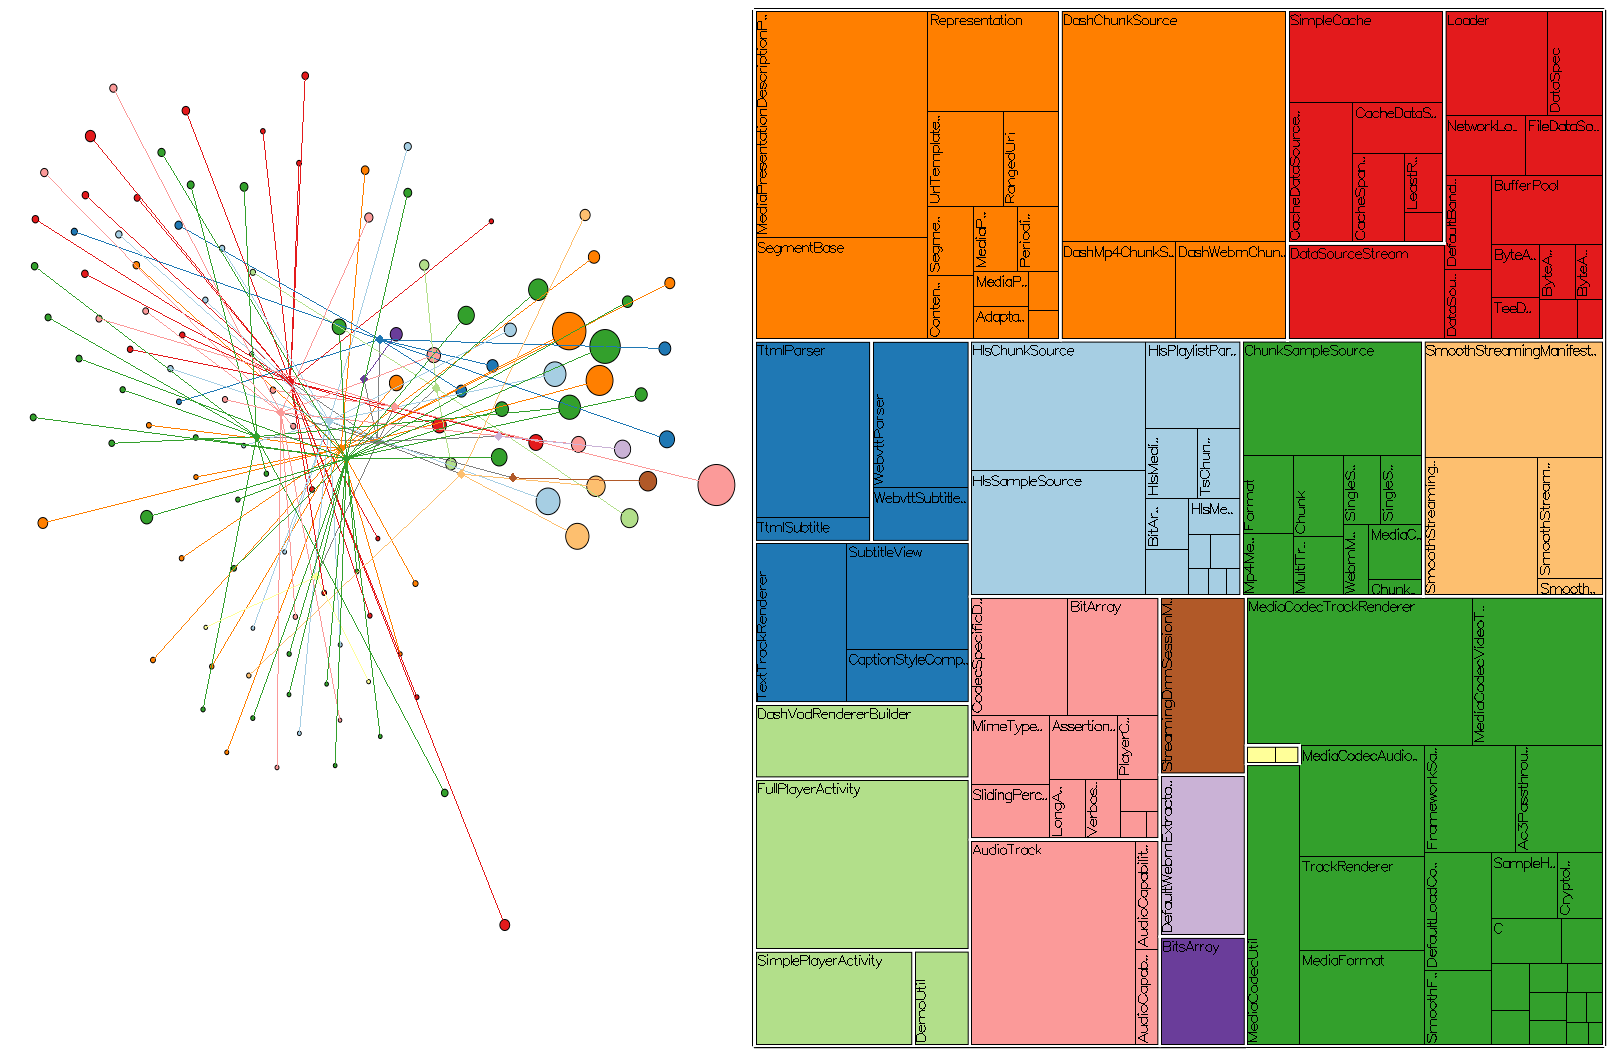
\includegraphics[width=1.0\textwidth]{figures/hier_sim_graph.png}
	\caption{Linking nodes hierarchically on the ExoPlayer project}
	\label{fig:hier_sim_graph}
\end{figure}


\begin{figure}[H]
	\centering
	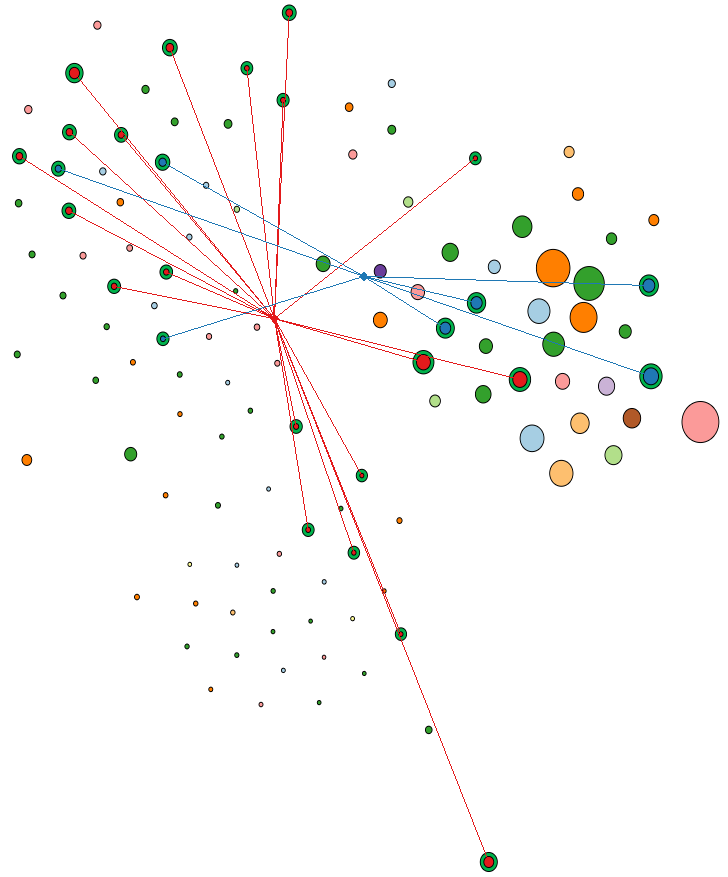
\includegraphics[width=0.7\textwidth]{figures/hier_two_sim_graph.png}
	\caption{Linking filtered packages hierarchically on the ExoPlayer project}
	\label{fig:hier_two_sim_graph}
\end{figure}

This experiment was an attempt to find correlation between similarity of classes and their location in th project structure. The conclusion we arrived at is that, for our datasets, there is none. Which is an interesting result nevertheless.

Our other goal was to encode similarity on the Treemap. In order to do so, we computed the $\mathbb{R}^{n}$ distances between every pair of points, selecting only the 1\% closest points. Between each pair in this set, we drew a line which uses the opacity to communicate the strength of the resemblance between the two points. The result for a single revision can be seen on figure \ref{fig:treemap_similarity}. It is interesting to see as the project evolves, how these relationships change.

\begin{figure}[H]
  \centering
  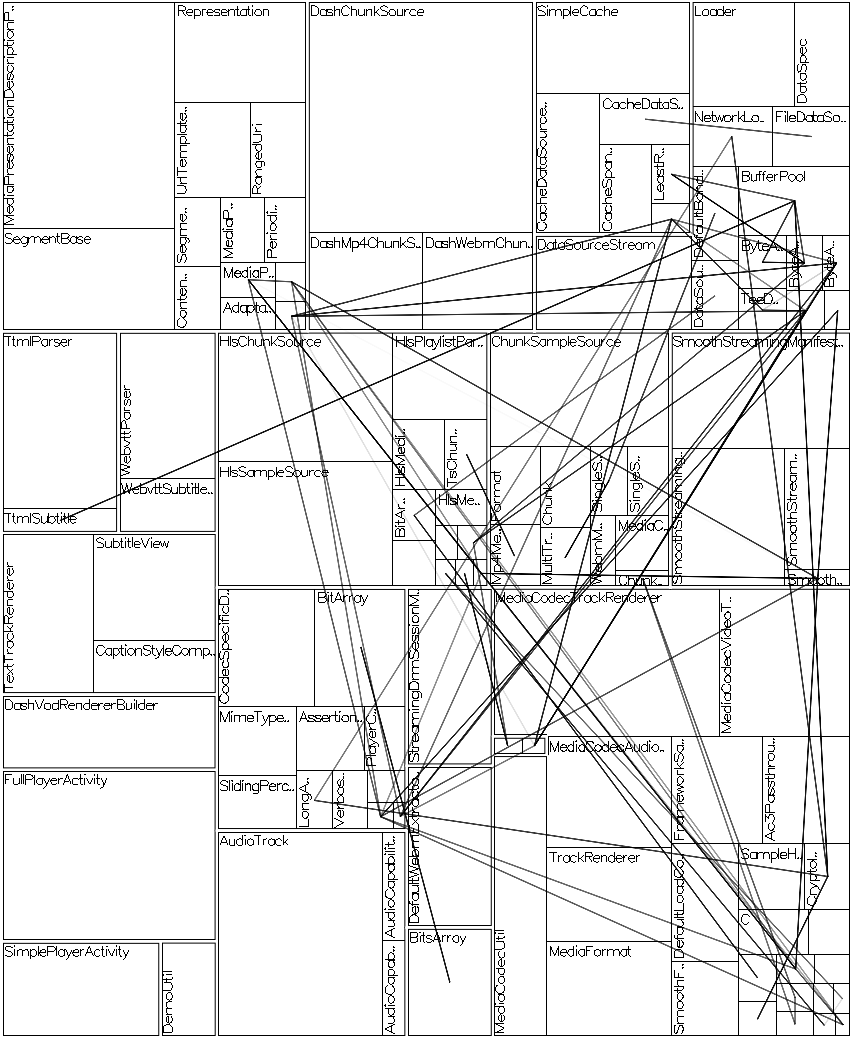
\includegraphics[width=0.7\textwidth]{figures/treemap_similarity.png}
  \caption{Linking nodes by similarity on the ExoPlayer project}
  \label{fig:treemap_similarity}
\end{figure}

One future improvement would be to use \citet{ref:holten06} approach with edge bundling to encode the similarity between nodes, as presented in figure \ref{fig:holten}.

\begin{figure}[H]
  \centering
  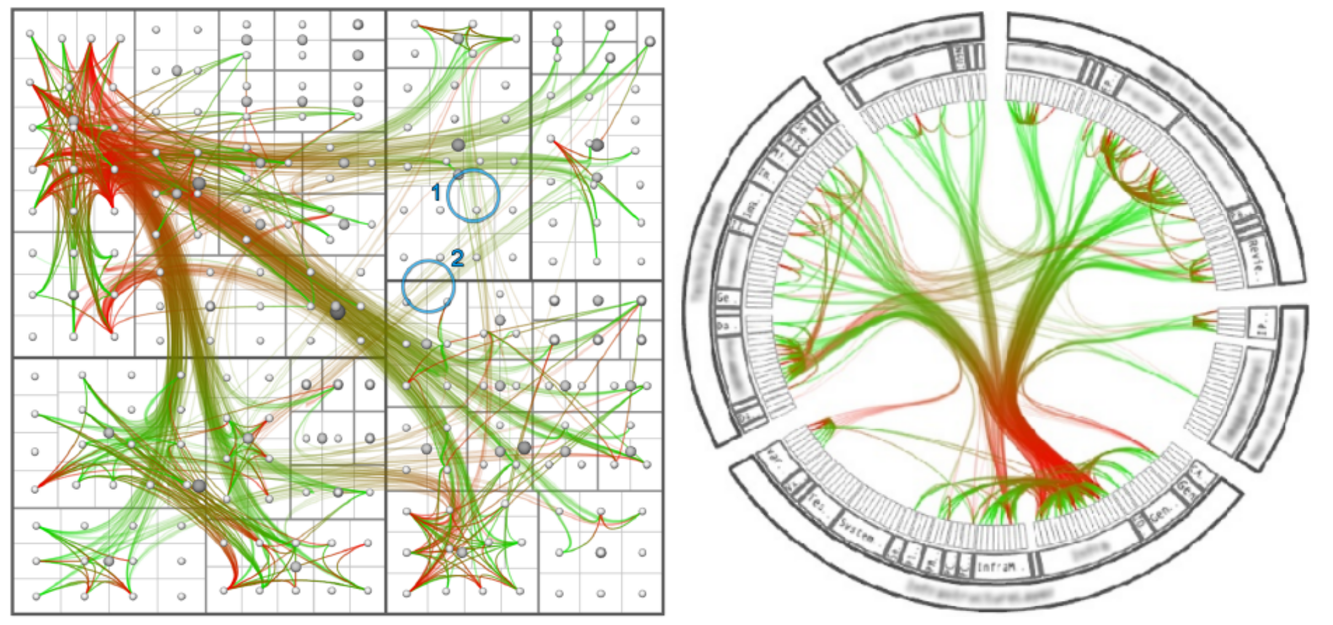
\includegraphics[width=1.0\textwidth]{figures/holten.png}
  \caption{Visualization of a software system's call graph with edge bundling}
  \legend{Source: \cite{ref:holten06}}
  \label{fig:holten}
\end{figure}
